\tikzset{every picture/.style={line width=0.75pt}}

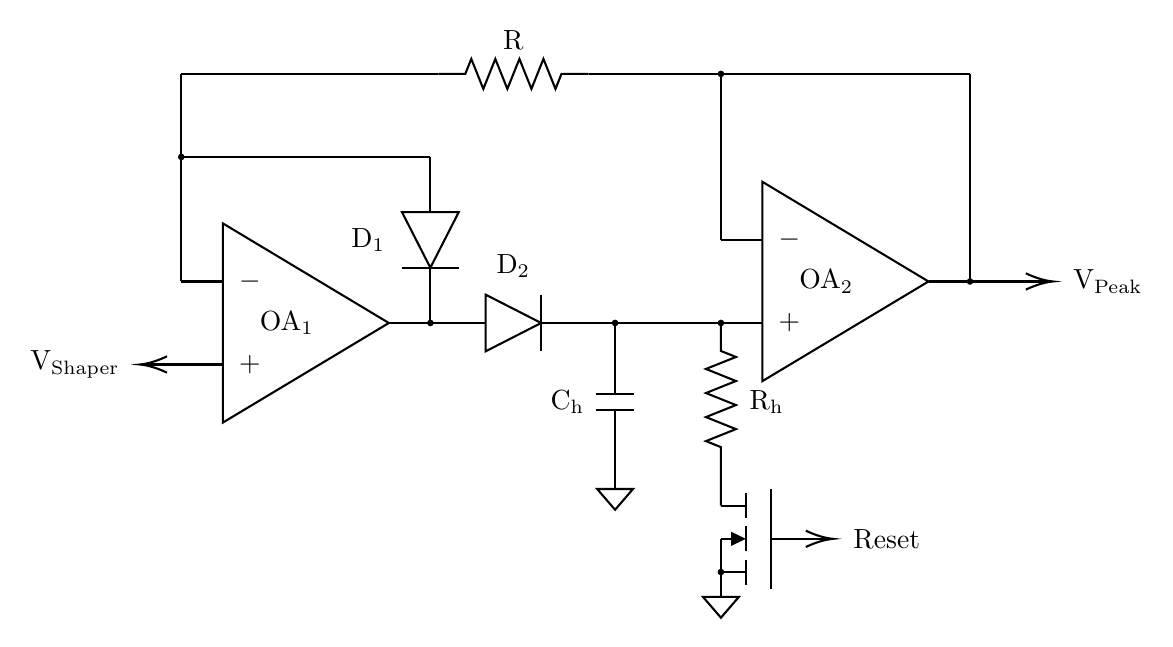
\begin{tikzpicture}[
    x=1.5pt, y=1.5pt, yscale=-1, xscale=1,
    every node/.style={font=\normalsize, inner sep=1pt}
]

%==================== Feedback resistor R (top rail) ====================
\draw    (200,40) -- (261.9,40) ;
\draw    (261.9,40) -- (268.41,40) -- (269.86,36.39) -- (272.76,43.61) -- (275.65,36.39) -- (278.55,43.61) -- (281.45,36.39) -- (284.35,43.61) -- (287.24,36.39) -- (290.14,43.61) -- (291.59,40) -- (298.1,40) ;
\draw    (298.1,40) -- (390,40) ;

%==================== OA_1 ====================
\draw    (210,76) -- (250,100) -- (210,124) -- cycle ;
\draw    (200,90) -- (210,90) ;
\draw    (210,110) -- (192,110) ;
\draw [shift={(190,110)}, rotate=0] [line width=0.75]
       (6.56,-1.97) .. controls (4.17,-0.84) and (1.99,-0.18) .. (0,0) .. controls (1.99,0.18) and (4.17,0.84) .. (6.56,1.97) ;
\draw    (200,40) -- (200,90) ;

%==================== D_1 (feedback diode) ====================
\draw    (200,60) -- (260,60) ;
\draw    (260,60) -- (260,73.31) ;
\draw    (266.83,73.31) -- (260,86.69) -- (253.17,73.31) -- cycle ;
\draw    (253.17,86.69) -- (266.83,86.69) ;
\draw    (260,86.69) -- (260,100) ;

%==================== D_2 (output diode) ====================
\draw    (250,100) -- (273.31,100) ;
\draw    (273.31,93.17) -- (286.69,100) -- (273.31,106.83) -- cycle ;
\draw    (286.69,93.17) -- (286.69,106.83) ;
\draw    (286.69,100) -- (340,100) ;

%==================== Hold capacitor C_h ====================
\draw    (304.5,100) -- (304.5,117) ;
\draw    (300,117) -- (309,117) ;
\draw    (300,121) -- (309,121) ;
\draw    (304.5,121) -- (304.5,140) ;
\draw    (300.19,140) -- (304.5,145) -- (308.81,140) -- cycle ;

%==================== Discharge resistor R_h ====================
\draw    (330,100) -- (330,106.74) -- (333.61,108.19) -- (326.39,111.08) -- (333.61,113.98) -- (326.39,116.88) -- (333.61,119.77) -- (326.39,122.67) -- (333.61,125.57) -- (326.39,128.46) -- (330,129.91) -- (330,144) ;

%==================== Reset MOSFET ====================
\draw    (336,141) -- (336,147) ;
\draw    (336,149) -- (336,155) ;
\draw    (336,157) -- (336,163) ;
\draw    (342,140) -- (342,164) ;
\draw    (342,152) -- (355,152) ;
\draw [shift={(357,152)}, rotate=180] [line width=0.75]
       (6.56,-1.97) .. controls (4.17,-0.84) and (1.99,-0.18) .. (0,0) .. controls (1.99,0.18) and (4.17,0.84) .. (6.56,1.97) ;
\draw    (330,144) -- (336,144) ;
\draw    (336,160) -- (330,160) ;
\draw    (330,152) -- (330,166) ;
\draw    (330,152) -- (334,152) ;
\draw [shift={(336,152)}, rotate=180] [fill={rgb, 255:red, 0; green, 0; blue, 0}, fill opacity=1] [line width=0.08] [draw opacity=0]
       (3.57,-1.72) -- (0,0) -- (3.57,1.72) -- cycle ;
\draw    (325.69,166) -- (330,171) -- (334.31,166) -- cycle ;

%==================== OA_2 ====================
\draw    (340,66) -- (380,90) -- (340,114) -- cycle ;
\draw    (330,40) -- (330,80) ;
\draw    (330,80) -- (340,80) ;
\draw    (380,90) -- (408,90) ;
\draw [shift={(410,90)}, rotate=180] [line width=0.75]
       (6.56,-1.97) .. controls (4.17,-0.84) and (1.99,-0.18) .. (0,0) .. controls (1.99,0.18) and (4.17,0.84) .. (6.56,1.97) ;
\draw    (390,40) -- (390,90) ;

%==================== Junction dots ====================
\fill (200,60)    circle (0.8) ;
\fill (260,100)   circle (0.8) ;
\fill (304.5,100) circle (0.8) ;
\fill (330,100)   circle (0.8) ;
\fill (330,40)    circle (0.8) ;
\fill (330,160)   circle (0.8) ;
\fill (390,90)    circle (0.8) ;

%==================== Labels ====================
% terminals
\draw (186,110) node [anchor=east] {V$_{\mathrm{Shaper}}$};
\draw (414,90)  node [anchor=west] {V$_{\mathrm{Peak}}$};
\draw (361,152) node [anchor=west] {Reset};

% op-amps
\draw (218,100) node [anchor=west] {OA$_{1}$};
\draw (213,90)  node [anchor=west] {$-$};
\draw (213,110) node [anchor=west] {$+$};
\draw (348,90)  node [anchor=west] {OA$_{2}$};
\draw (343,80)  node [anchor=west] {$-$};
\draw (343,100) node [anchor=west] {$+$};

% passives
\draw (280,35)  node [anchor=south] {R};
\draw (250,80)  node [anchor=east]  {D$_{1}$};
\draw (280,90)  node [anchor=south] {D$_{2}$};
\draw (298,119) node [anchor=east]  {C$_{\mathrm{h}}$};
\draw (336,119) node [anchor=west]  {R$_{\mathrm{h}}$};

\end{tikzpicture}